\documentclass[12pt,letterpaper]{article}
\usepackage{color, graphicx}
\usepackage[pdftitle={Turing Machine Simulator}, pdfauthor={L3}, colorlinks=true, urlcolor=blue]{hyperref}
\usepackage{listings}
\definecolor{verbgray}{gray}{0.9}

\lstnewenvironment{code}{%
	\lstset{backgroundcolor=\color{verbgray},
		frame=single,
		framerule=0pt,
		basicstyle=\ttfamily,
		columns=fullflexible}}{}

%opening
\title{Turing Machine Simulator User Manual}
\author{Brian Ward and David Kocen}
\date{\today}

\begin{document}

\maketitle
\begin{center}
	
\includegraphics{images/icon.png}
\end{center}
\pagebreak
\tableofcontents

\pagebreak

\section{About Turing Machines}

\noindent Originally proposed by Alan Turing in 1936, a Turing Machine is an abstract machine that allows for the simulation of any computational algorithm. The machine works on an infinite tape made up of discrete cells. When started, the machine head first looks at the starting cell and reads the symbol in that cell. Then, based on user defined instructions the machine replaces the symbol in the cell with a symbol from the machine's alphabet (it can be the same symbol) and then moves the head either left or right. This process continues until the machine reaches a predefined halt state. The user can then read the contents of the tape to get the output of the program.\\

\noindent Despite their simplicity, Turing Machines are believed to be capable of computing any paper and pen algorithm performed by a human, as stated in the Church-Turing Thesis. As such, anything that can be performed on a modern day computer can be simulated on a Turing Machine. However, that is not to say that Turing Machines, and thus modern computing, are without any weaknesses. Like all computational models, Turing Machines are subject to the Halting Problem. The problem asks if there is a general algorithm for determining if a given program will eventually halt. With the creation of Turing Machines, Alan Turing proved that there is no general algorithm to solve the halting problem. The implications of this a far reaching and point out some of the fundamental limitation of computers as a whole.\\ 

\noindent Turing Machines are probably the most well known models of computation that are capable of performing all tasks that a modern computer can perform. However, there are a number of other equivalent models. These include lambda calculus, counter machines, and FRACTRAN. All of these models, including Turing Machines, are classified as Turing-Complete. From Turing Machines came the explosive growth of computers and the field of computer science. These simple yet powerful machines provide incredible insight into the field of computing and what it can and cannot solve for us.

\section{Using the Simulator}

\subsection{Overview}
	\noindent This Turing Machine simulator provides all the functionality of a bidirectional, infinite tape Turing Machine with the qualifier that the simulated machine does not actually have an infinitely long tape (though it is plently long for all practical uses). This is due to fundamental memory limitations in computers. In addition to simulating a Turing Machine, this program is also capable of simulating a unidirectional, infinite tape Turing Machine and a two-tape Turing Machine. These different machines can be viewed as both simulated tapes and as texts providing information for each step. Within the program itself, the user can write the various states and state changes that the machine should follow. These can then be saved as .tm files and loaded into the simulator for use at a later time.
	
\begin{figure}[hbt!]
	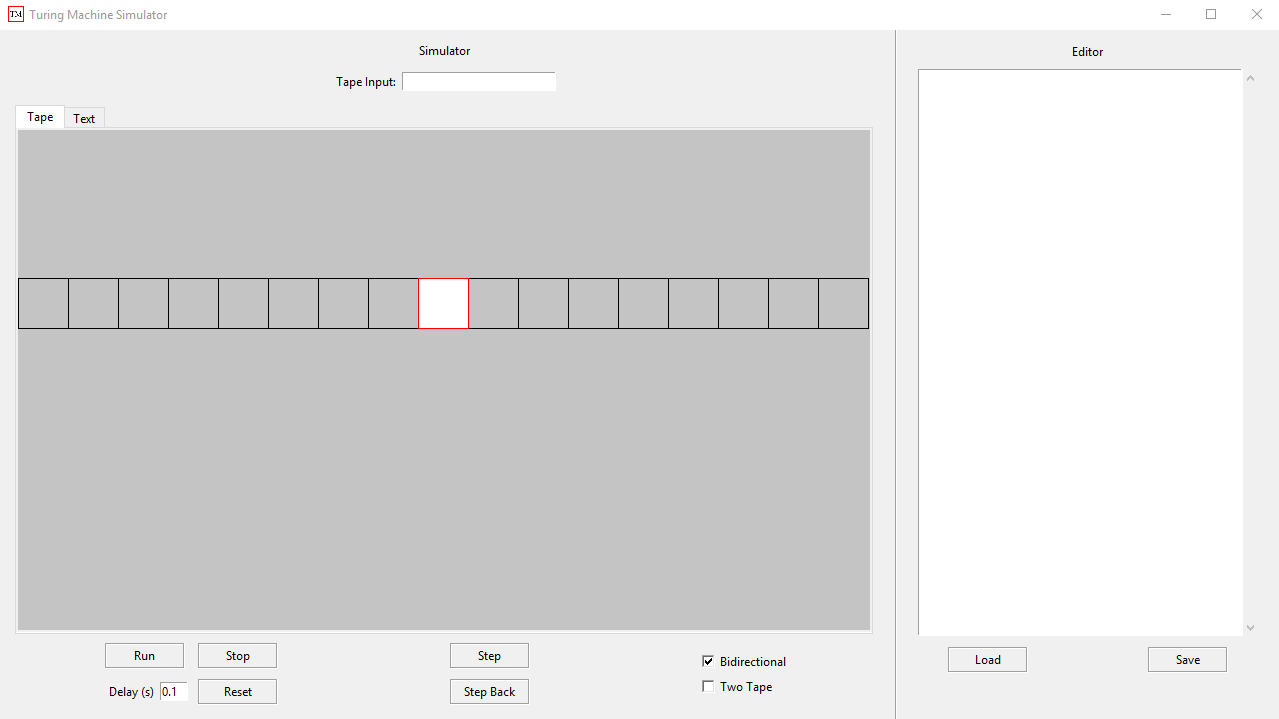
\includegraphics[scale=.4]{images/simulator_blank.png}
	\caption{Simulator upon startup}
\end{figure}

\subsection{Running the Program}
	\noindent In order to run this program you must have either Python 2.7 or 3.7 installed on your computer. Additionally, if you are running this program on a Linux machine you will need to install the TKinter library for your installation of Python. After installing the prerequisite software, simply double click \texttt{TMGUI.py} or run \texttt{TMGUI.py} in the command line.

\subsection{The Editor}
	\noindent The editor window is located on the right of the program window. Here is where you will load, write, and save .tm files that will define the functionality of your Turing Machine.
	
	\subsubsection{Writing a .tm file}
	\noindent The instructions for the simulated Turing Machine are written as a .tm file. These can be created by either using the editor within this program or creating an ordinary text file and saving it with the extension .tm. Instructions are written in the following format:
	\begin{itemize}
		\item States are always integers with 0 being the initial state.
		\item -1 denotes a halt-and-accept state, -2 is a halt-and-reject state, and -3 is a general halt state. All other state number must be nonnegative.
		\item L tells the machine to move left and R tells it to move right. Additionally, if you are writing a two tape Turing Machine, S tells the machine to stay where it is. S can only be used for two tape Turing Machines.
		\item A capital 'B' represents the blank symbol.
		\item For a one tape Turing Machine, each line of the .tm file takes the form \\ STATE  SYMBOL  NEW-STATE  NEW-SYMBOL  DIRECTION.\\ So the line 
		\begin{center}
			2 b 5 c L 
		\end{center}
		tells the machine that if it is in state 2 and is reading the symbol b, replace the b with a c, move left, and change to state 5.
		\item To include comments start each comment line with a \#.
		\item For a two tape Turing Machine, each line of the .tm file takes the form STATE SYMBOL1:SYMBOL2 NEW-STATE NEW-SYMBOL1:NEW-SYMBOL2  DIRECTION1:DIRECTION2.\\ So the line
		\begin{center}
			0 a:b 3 B:a L:S
		\end{center}
		tells the machine that if it is in state 2 and is reading the symbol a in tape 1 and b in tape 2, replace the a in tape 1 with a blank and the  b in tape 2 with an a, move tape 1 left but do not move tape 2, and change to state 3.
		\item If there is no specification for a given state and character combination the machine will enter a halt-and-reject state.
	\end{itemize}
	
	\subsubsection{Saving a .tm file}
	\noindent If you have written your machine instructions within the editor window, you can save them to your computer in order to use them at another time. To do so: \begin{enumerate}
		\item Ensure that your instructions follow the exact format described above. While anything you write in the editor window can be saved as a .tm file, if it does not follow the proper format the simulator will be unable to run.
		\item Click the save button located at the bottom right of the editor section.
		\item Choose the directory you wish to save the file in, provide a file name, and then click save.
	\end{enumerate}
	This will create a .tm file in the given directory that can be used at a later date.
	
	\begin{figure}[hbt!]
		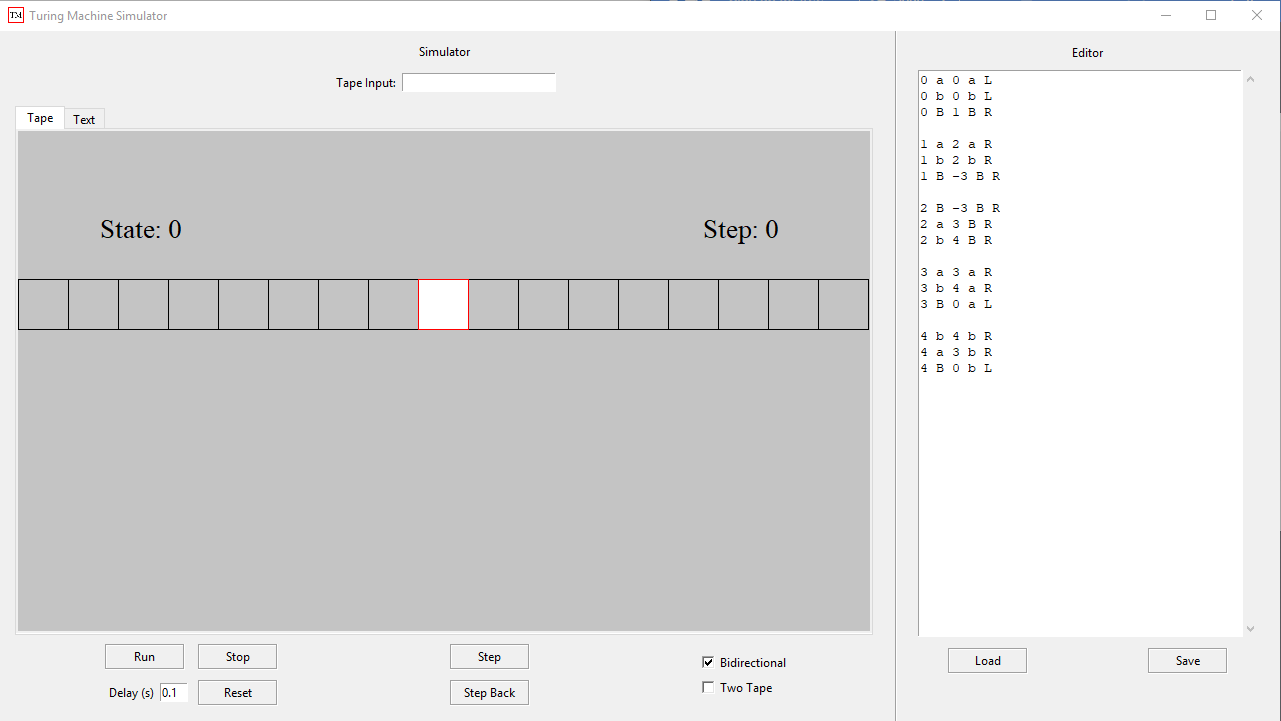
\includegraphics[scale=.4]{images/simulator_loaded.png}
		\caption{Simulator with loaded .tm file}
	\end{figure}

	\subsubsection{Loading a .tm file}
	\noindent To load a previously used .tm file:
	\begin{enumerate}
		\item Click the load button located at the bottom left of the editor section.
		\item Navigate to your file, select it, and click open.
	\end{enumerate}
	You should now see the list of instructions for your Turing Machine in the editor window. You can then edit them as you see fit and save them just like anything else that is written in the editor window.\\

\subsection{The Simulator}
\noindent The simulator window is located on the left side of the program window. Here is where you can see a visualization of your Turing Machine running both graphically and as text.
	\subsubsection{Reading the Simulator}
	In this program there are two ways you can simulate the Turing Machine. This is either as a graphical representation of the tape or as text. At any time in the machines run you can go between seeing the machine simulated as an actual tape and seeing it as text. This is done by toggling between the ``tape" and ``text" tabs located at the top left of the simulator window.\\
	
	\noindent When simulating the machine as a tape:
	\begin{itemize}
		\item The current state and step are located above the tape itself.
		\item The cell currently being read by the machine is the white cell 
	\end{itemize}
	
	\noindent When simulating the machine as text:
	\begin{itemize}
		\item Each step is written as a chunk of text with the current step, the current state, and what is currently written on the tape.
		\item The letter with a caret beneath it is the one being read by the machine
	\end{itemize}

	\noindent While the ``tape" tab is useful for getting a visual understanding of how your Turing Machine runs, we recommend doing any actual analysis in the ``text" tab since you are limited to only ever seeing a section of the entire tape in the ``tape" tab whereas you can easily scroll through all the steps when in the ``text" tab.
	
	\subsubsection{Running a Turing Machine}
	\noindent In order to run a Turing Machine do the following:
	\begin{enumerate}
		\item Either load a .tm file into the editor or save what you have written to your machine. Whenever a machine is loaded in the simulator, you will then see a ``state" and ``step" label appear in the tape and text window.
		\item If your .tm file is written for a unidirectional Turing Machine, uncheck the ``Bidirectional" box located at the bottom right of simulator window. If your .tm file is written for a two tape Turing Machine, check the ``Two Tape" box located directly below the ``Bidirectional" box. If you do not check off the proper boxes the simulator will likely halt and reject any input, but could also attempt\footnote{See Section \ref{halt}} to run forever. Note that these options are mutually exclusive, the simulator does not support two tape unidirectional Turing Machines.
		\item Type in the textbox labeled ``Tape Input" located in the top center of the simulator window what you want the initial tape input to be.
		\item Enter the delay you want between each step in the textbox labeled ``Delay" located in the bottom left of the simulator window. The default delay is 0.1s
		\item Click the run button located directly above the ``Delay" textbox. 
		\item If you wish to stop the run at any time press the ``Stop" button located to the right of the ``Run" button. If you wish to reset the machine click the ``Reset" button located directly below the ``Stop" button.
	\end{enumerate}

	\begin{figure}[hbt!]
		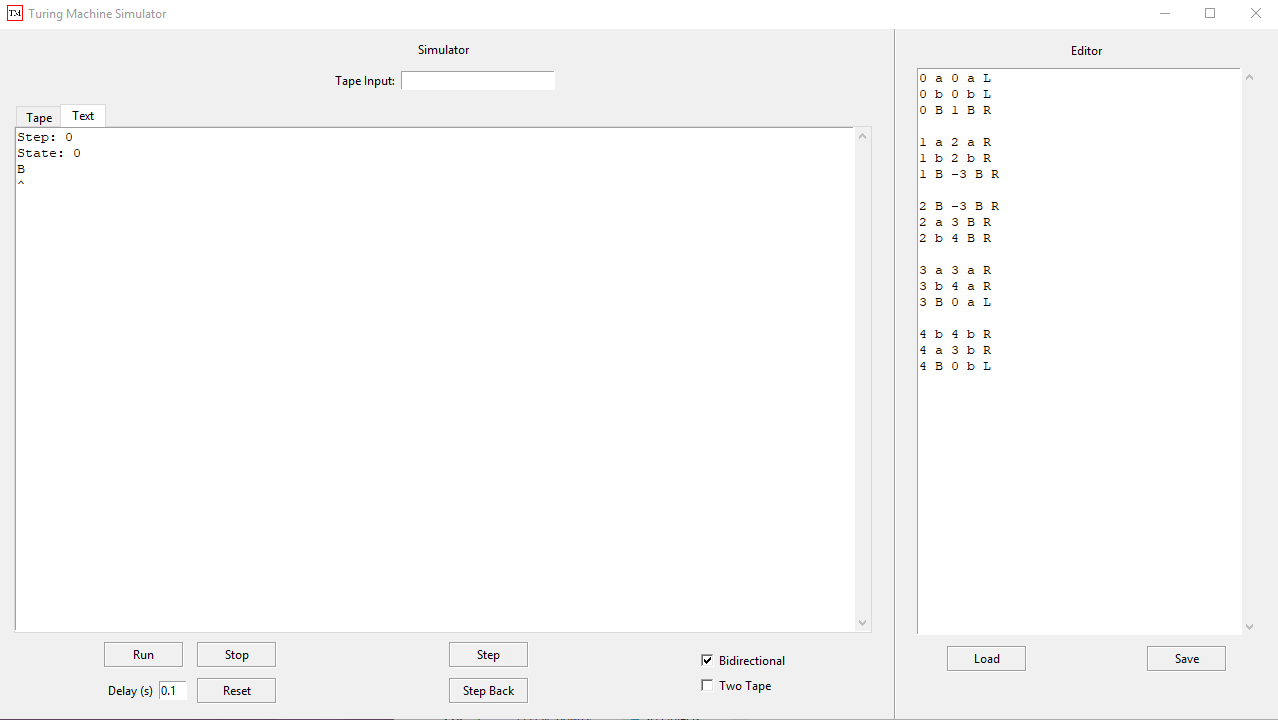
\includegraphics[scale=.4]{images/simulator_text.png}
		\caption{Simulator in text tab}
	\end{figure}

	\subsubsection{Going Step by Step Through a Run}
	\noindent If you wish to have more control over the run of your Turing Machine, you can go through step by step using the ``Step" and ``Step Back" buttons located at the bottom center of the simulator window. Note that if you press the ``Step Back" button at step 0 nothing will occur. If you press the ``Step" button after the machine has halted you will be adding additional steps but the machine will stay in a halt state. These functionalities can be used in conjunction with the ``Run" and ``Stop" functionality, as expected. 
	
	\subsubsection{Encountering the Halting Problem}\label{halt}
	\noindent Because of fundamental limitations to Turing Machines and computation, it is impossible to know if your Turing Machine will ever halt. This is the Halting Problem and is discussed in the ``About Turing Machines" section. If you run a Turing Machine that never halts the program will likely become unresponsive. At this point we recommend closing and restarting the program. Alternatively, to help deal with this problem we have set the maximum number of steps allowed for any given run to be 200,000 steps. After the program has determined all of these steps it should respond again and show the run for 200,000 steps. This may take a while so restarting the program is probably your best option. 

\section{Using Grapher}
In addition to simulating a Turing Machine, we have included a program that automatically converts a .tm file into an easy to follow directed graph. This is useful if the user wishes to have a visual representation of the Turing Machine without actually having to test various input strings. To use the grapher do the following:
\begin{enumerate}
	\item Install the graphviz Python library using the command \texttt{pip install graphviz}.
	\item Download the Graphviz program \href{https://www.graphviz.org/download/}{here}. Make sure that you follow all installation instructions  (Including adding this program to your PATH on Windows systems) 	or else the grapher will not be able to work.
	\item Open the grapher by running \texttt{grapher.py}.
	\item Click the graph button and select the .tm file you wish to graph. The program will automatically make a .png of the Turing Machine and save it in a directory titled img within the same directory that \texttt{grapher.py} is located in.
\end{enumerate}
The Grapher was developed with the sole intent of graphing the .tm files associated with one-tape Turing Machines. It will function with two-tape files, but the output may not be as readable or look as expected.

\begin{figure}[hbt!]
	\centering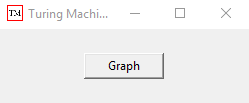
\includegraphics[scale=.7]{images/grapher.png}
	\caption{Grapher upon startup}
\end{figure}
	
\section{Technical Overview}
The simulator code is divided into two classes. The first of these classes is \texttt{turing\_machines.py}. This class serves as the backend for the simulator, housing objects which model the Turing Machines. It is here that the actual code for simulating a Turing Machine is contained. The code in this class is adapted from the simulator created by \href{http://www.cs.bc.edu/~straubin/}{Howard Straubing}. The other class is \texttt{TMGUI.py}. This class is a GUI built using the Python library TKinter and allows for the user to actually interact with the program. Additional documentation can be found within these classes.\\

\noindent The grapher code uses GraphViz, a program for generating directed graphs, in order to convert a .tm file into a directed graph of the state transitions. This code was initially developed in order to provide a nice animation for Turing Machines to be included within the simulator itself. However, to provide this functionality would require additional libraries and is particularly slow. As such, we decided to devote most of our efforts on exploring two tape Turing Machines and included the grapher as a standalone `bonus' program.

\subsection{Functional Limitations}
	\noindent There are a number of different functional limitations to the simulator program. 
	\begin{itemize}
		\item We have capped the maximum number of steps at 200,000 in order to help deal with the Halting Problem. We feel this is more than enough steps for most simulations though if more are needed the user can edit the \texttt{MAX\_STEPS} variable in \texttt{turing\_machines.py}.
		\item Because of limitations in computer memory the tape used is not actually infinite. Each tape is limited to 20,000 spaces. The simulator will not let you move past \textit{either} end of the tape -- attempting to do so will simply keep the head position the same. This is particularly important to keep in mind when simulating one-way `infinite' tapes, as the head starts at the left end of the tape.
		\item Unidirectional tapes are not an option when using a two tape Turing Machine despite theoretically being possible. This decision was made mainly because this model does not seem to provide any more value or insight -- it would be rather trivial to adapt the existing code to handle it if truly desired.
		\item Due to how the TKinter Canvas object works, it is not possible to scroll through what is written on the tape when in the ``tape" tab. You are limited to only a section of the entire tape, centered on the reading head. As stated earlier, we recommend using the ``text" tab if a fuller view is desired.
	\end{itemize}

\subsection{Known Issues}
	\noindent The only known issue right now is the program begins to lag if too large of a tape input is entered, or if the program is run for a long time on many machines or on many different inputs. It is unclear if this is due to a memory leak within our program or a limitation on the part of Python, though considerable effort was put in to mitigate this problem. Restarting the program resolves this lag. 
\newpage

\appendix
\section{Sample .tm file}\label{sample}
A .tm file defining a unidirectional Turing Machine for reversing tape input.
\begin{code}
#Phase 0: Mark the first entry. a is 0, b is 1
0 0 1 a R
0 1 1 b R
0 B -3 B R
#Phase 1:  Move forward to first blank and write #
1   1   1   1  R
1   0   1   0  R
1   B   2   #  L
#Phase 2:  Move left until you find 0, 1 or blank
2   0   3   X  R
2   1   4   X  R
2   B   5   B  R
2   X   2   X  L
# 2.1: If you found the first character, replace with a blank
2   a   3   B  R
2   b   4   B  R
#Phase 3a:  Found 0, move right to blank, then left to #
3   0   3   0  R
3   1   3   1  R
3   X   3   X  R
3   #   3   #  R
3   B   6   0  L
6   0   6   0  L
6   1   6   1  L
6   #   2   #  L
#Phase 3b, Found 1
4   0   4   0  R
4   1   4   1  R
4   X   4   X  R
4   #   4   #  R
4   B   6   1  L
#Cleanup phase
5   X   5   B  R
5   #   -3  B  R
\end{code}

\section{Sample Grapher Output}
\begin{figure}[hbt!]
	\centering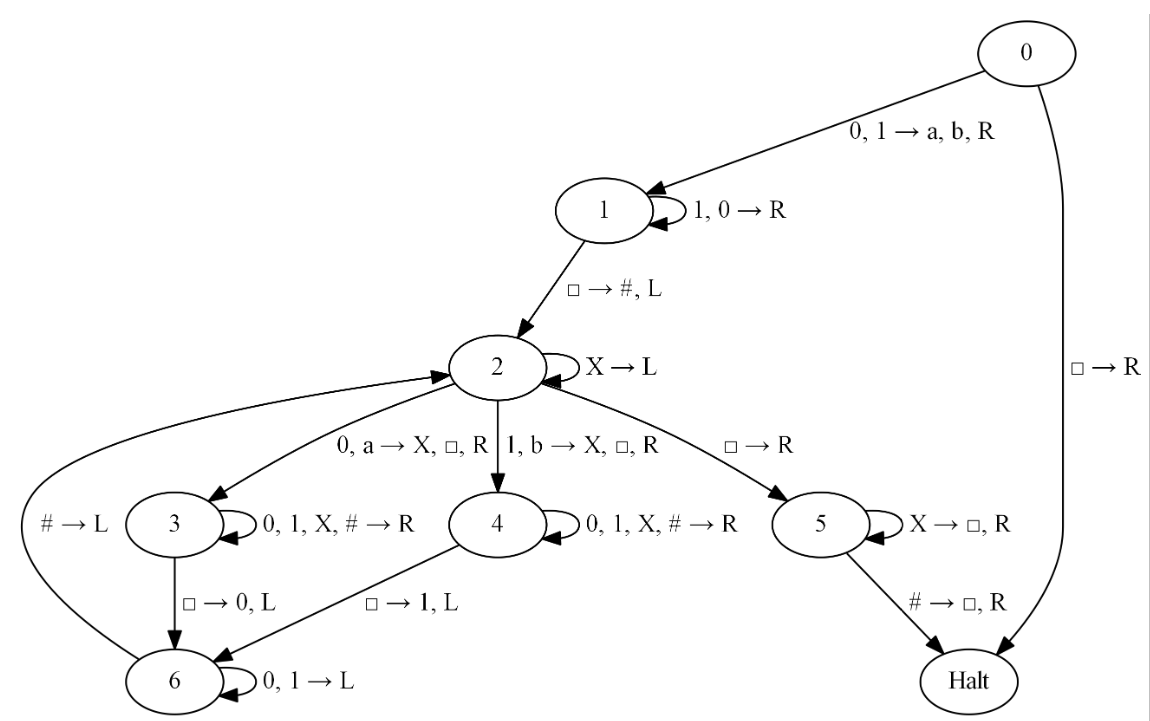
\includegraphics[scale=.5]{images/sample_graph.png}
	\caption{Directed graph of the sample .tm file from Appendix \ref{sample}}
\end{figure}


\end{document}
